\documentclass[11pt,a4paper]{scrarticle}
\usepackage[utf8]{inputenc}
\usepackage{cmap}
\usepackage[T2A]{fontenc}
\usepackage[russian]{babel}
\usepackage{amsmath,amssymb,amsthm,mathtools}
\usepackage{array}

\usepackage{indentfirst}
\usepackage{xcolor,graphicx, tikz, wrapfig}
\usepackage{longtable}
\usepackage{placeins}

\usepackage{minted}
\usemintedstyle{vs}

\usepackage[left=2cm,right=2cm,top=2cm,bottom=2cm,bindingoffset=0cm]{geometry}

\usepackage[unicode]{hyperref}
\definecolor{linkcolor}{HTML}{0000E6}
\definecolor{urlcolor}{HTML}{0000E6}
\definecolor{citecolor}{HTML}{0000E6}
% \hypersetup{pdfpagemode=None,linktoc=page,citecolor=citecolor,linkcolor=linkcolor,urlcolor=urlcolor,colorlinks=true}

\theoremstyle{definition}
\newtheorem{subtask}{Пункт}

\DeclareMathOperator*{\argmax}{arg\,max}
\DeclareMathOperator*{\argmin}{arg\,min}
\newcommand{\floor}[1]{\left\lfloor #1 \right\rfloor}
\newcommand{\ceil}[1]{\left\lceil #1 \right\rceil}


\setlength{\parindent}{1cm}

\author{Клычков Максим Дмитриевич}

\begin{document}

\centerline{\textbf{\huge Алгоритмы и структуры данных-2}}
\centerline{\textbf{SET 5. Задача A1.}}
\begin{flushright}
    \emph{Весна 2024. Клычков М. Д.}
\end{flushright}

\begin{figure}[htp]
    \centering
    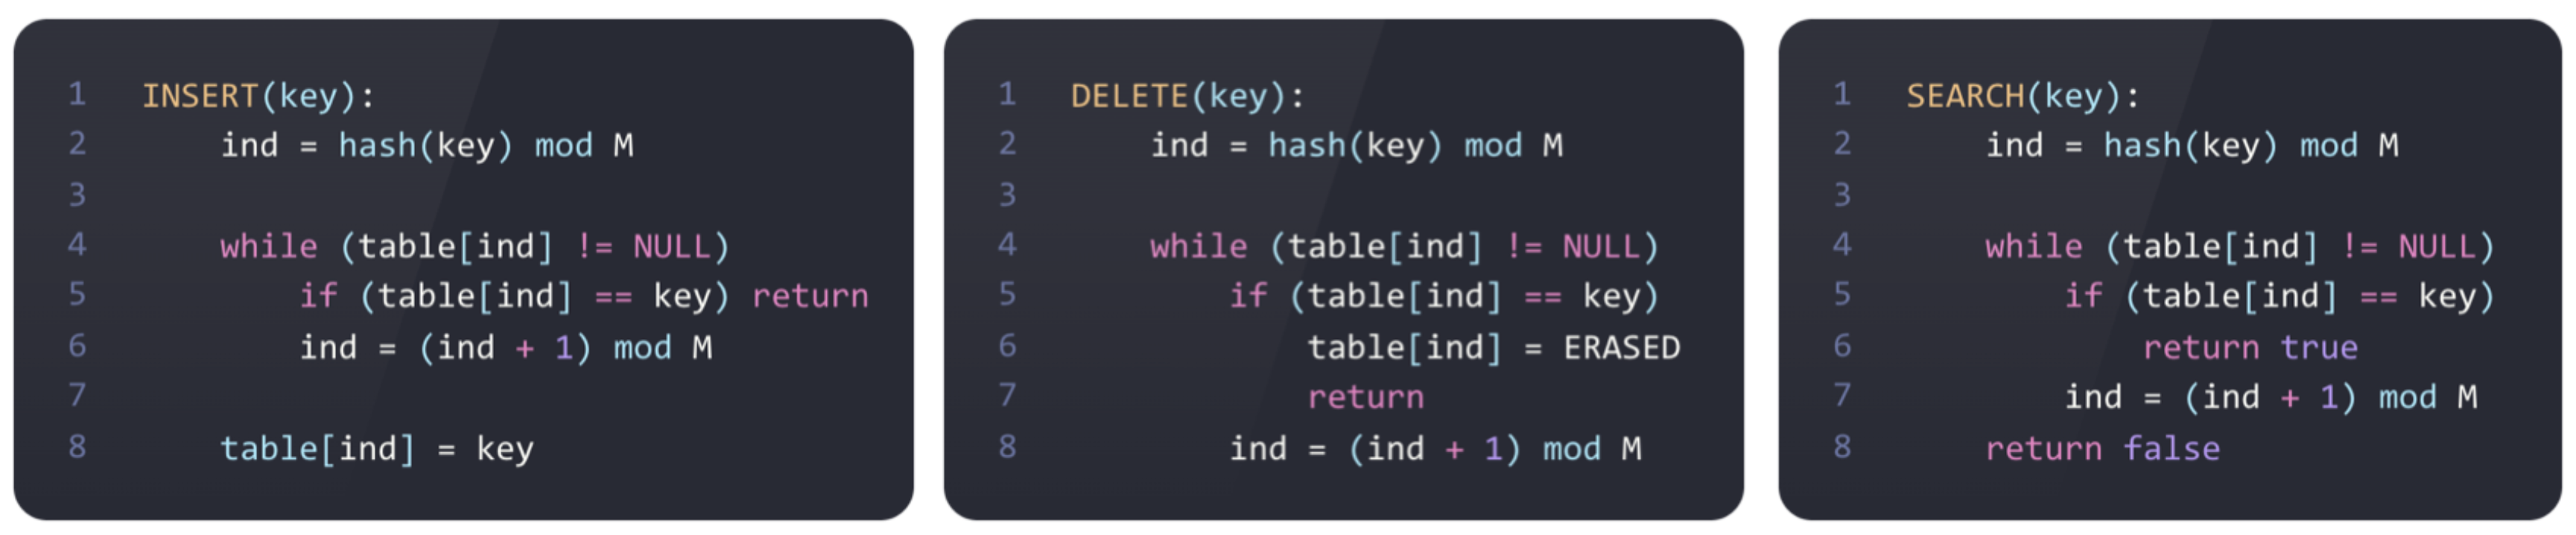
\includegraphics[width=\textwidth]{static/code.png}
    \caption{Код из условия}
    \label{fig:code}
\end{figure}

\begin{subtask}
    Сразу заметим, что в методе \texttt{INSERT} не происходит проверки на переполнение хеш-таблицы, а соответственно, можно предположить, что не происходит и перехеширования (предполагаем, что структура данных содержит только приведенные в условии методы). Это сразу заставляет задуматься о \textbf{переполнении} хеш-таблицы.

    Например, последовательная вставка элементов, хеши которых полностью покрывают отрезок возможных значений хеш-функции $[0; m - 1]$. Такими вставками мы добьемся такого состояния хеш-таблицы, при котором невозможно вставить новое значение. Конкретный пример:
    при ключе \texttt{int} и хеш-функции $h(key) = (key \mod m)$ выполняем вставки
    $$\texttt{INSERT}(0), \texttt{INSERT}(1), \dots, \texttt{INSERT}(m - 1).$$
    Теперь при последующей вставке $\texttt{INSERT}(m)$ произойдет зацикливание.

    Более того, учитывая несовершенность условия цикла \texttt{while} метода \texttt{INSERT} мы войдем в бесконечный цикл, зацикленно пробегая по всем ячейкам хеш-таблицы, так как условие выхода из цикла
    \mint{cpp}|table[ind] == nullptr|
    \noindent никогда не выполнится.

    Заметим, что аналогичная проблема зацикливания при заполненной хеш-таблице свойственна и другим двум методам структуры: \texttt{DELETE} и \texttt{SEARCH}. Возможное решение этой проблемы будет приведено в \textbf{Пункте 2}.

    Еще один источник потенциальных проблем — значение \texttt{ERASED} удаленных элементов структуры. Снова обратимся к методу \texttt{INSERT}: при поиске свободной ячейки для вставляемого элемента не учитывается \texttt{ERASED}. Таким образом, «умершие» элементы продолжают хранится в хеш-таблице до полного ее уничтожения, занимая память, которая может быть переиспользована для новых элементов структуры.

    Приведем конкретный пример: заполним хеш-таблицу тем же образом, что и в примере выше. Теперь, имея полностью заполненную хеш-таблицу последовательно выполним удаления:
    $$\texttt{DELETE}(0), \texttt{DELETE}(1), \dots, \texttt{DELETE}(m - 1).$$
    Несмотря на то что все элементы были удалены и логический размер структуры равен $0$, любая вставка, удаление или поиск введут программу в бесконечный цикл.
\end{subtask}

\begin{subtask}
    Сначала поборемся с проблемой зацикливания, которая происходит в каждом из приведенных методов. Предлагается обходить таблицу при помощи цикла \texttt{for} вместо \texttt{while} с целью ограничить максимальное количество шагов цикла. Будем итерироваться по переменной \texttt{diff}, которая принимает значения в полуинтервале $[0;m)$, и получать очередной индекс \texttt{ind} как сумма хеша и \texttt{diff} по модулю \texttt{M}.

    Ниже в качестве примера приведена исправленная функция \texttt{SEARCH} на \texttt{C++} (остальные функции должны быть исправлены аналогично):

    \begin{minted}
    [
    frame=lines,
    framesep=2mm,
    baselinestretch=1.2,
    fontsize=\footnotesize,
    linenos
    ]
    {cpp}
bool Search(int key) const {
    auto hash = Hash(key);

    for (int diff = 0; diff < m_; ++diff) {
        int i = (hash + diff) % m_;

        if (table_[i] == nullptr) {
            return false;
        }
        if (table_[i]->key == key) {
            return true;
        }
    }
    return false;
}
    \end{minted}

    Теперь решим проблему, связанную с \texttt{ERASED}. Перепишем код \texttt{INSERT} так, чтобы запись в ячейки \texttt{ERASED} была разрешена.

    \begin{minted}
    [
    frame=lines,
    framesep=2mm,
    baselinestretch=1.2,
    fontsize=\footnotesize,
    linenos
    ]
    {cpp}
bool Insert(int key) {
    auto hash = Hash(key);

    for (int diff = 0; diff < m_; ++diff) {
        int i = (hash + diff) % m_;

        if (table_[i] == nullptr || table_[i] == ERASED) {
            table_[i] = new KeyValT(key);
            return true;
        }
    }
    return false;
}
    \end{minted}

\end{subtask}

\end{document}

